\section{Trainingsvorgang}

Der Trainingsvorgang basiert auf ein mehrschichtiges tiefen neuronalen Netzwerks. Das Netzwerk aus Neuronen besteht aus drei Schichten:
\begin{description}
	\item Input-Schicht
	\item Hidden-Schicht 
	\item Output-Schicht
\end{description}
Die Input-Schicht stellt dabei die Eingangsdaten dar, welche als Trainingsmaterial dient. Bei diesen Daten handelt es sich um Sprachaufnahmen. Bei Bedarf können diese Sprachaufnahmen dementsprechend vorverarbeitet werden, wie zum Beispiel durch Einsatz von Filtern. Anschließend können die Daten in die Netztopologie eingespeist werden. Eine Vorklassifizierung der Sprache führt zu einer Erhöhung der Spracherkennungsrate von mehreren Sprachen. In der Hidden-Schicht geschieht das eigentlich Training. Dabei wird die Sigmoid-Funktion als Aktivitätsfunktion eingesetzt. Diese Funktion beschreibt den Korrelation zwischen Input-Wert und  Aktivitätslevel eines Neurons dar. Dabei wird der Netzinput auf die X-Achse eingetragen. Auf die Y-Achse wird der zugehörige Aktivitätslevel eingetragen. Der Aktivitätslevel wird durch eine Ausgabefunktion dann in den Output transformiert, den das Neuron an andere Neuronen weitersendet\cite{Neuronal31:online}. Das Netz wird beginnend von der Input-Schicht bis Output-Schicht vollständig durchlaufen. 
\begin{equation}
sigm(x)=\frac{ 1 }{1+e^{-x}  }
\label{normal}
\end{equation}
Sobald die Output-Schicht erreicht ist, wird das Netz rückwärts durchlaufen. Dieses Verfahren wird auch Gradientenabstiegsverfahren genannt und wird benötigt, um fehlerhafte Kantengewichte herauszufinden und anzupassen. Die Kantengewichte des Netzes werden anfangs mit null initialisiert, sodass die Kantengewichtungen korrigiert werden müssen. Die Ableitung der Sigmoid-Funktion kommt bei der Korrekturberechnung zum Einsatz \ref{ableitung}. Diese Funktion ist für eine geringe Datenmenge geeignet. Bei größeren Datenmengen entsteht ein Nachteil, welches sich auf die Wissensausprägung des Netzes auswirkt. Beim Rückwärts durchlaufen entsteht ein Wissensverlust \cite{bishop.2006}. Dieser Verlust wird durch das Maxima der Ableitung der verwendeten Funktion repräsentiert. Dieser kann bis zu 25 \% betragen. Der entstehende Verlust würde die Klassifizierungsrate des Trainingsmodels reduzieren, welches in Abbildung \ref{fig:features11.0} dargestellt ist \cite{Kulbear.2017}.
\begin{equation}
sigm(x)'= \frac{ e^{x} }{(e^{x} +1)^2  }
\label{ableitung}
\end{equation}

\begin{figure}[h!]
	\centering
	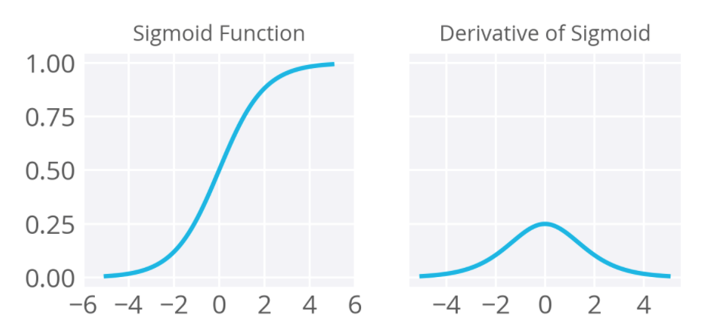
\includegraphics[width=1.0\linewidth]{images/sigmund}
	\caption{Darstellung der Sigmoid-Funktion und dessen Ableitung \cite{Kulbear.2017}} %Generelle
	\label{fig:features11.0}
\end{figure}
Anstelle der Sigmoid-Funktion wird in den Deep-Learning-Netzen Rectified linear Units ($ReLUs$) verwendet. Diese Funktion ist dem menschlichen Neuron am ähnlichsten und bringt zudem eine erhöhte Verarbeitungsgeschwindigkeit mit sich \cite{zeiler.2013}. 
\begin{equation}
y_{j} = ReLU(x_{j}) = max(0,x_{j}) 
\label{eq:ReLU}
%\caption{Rectiefied linear Units als Aktivierungsfunktion}
\end{equation}
\begin{equation}
x_{ j } = b_{ j } + \sum{ }{ }{ x_{ ij } * y_{j}}
\label{eq:Gewichte}
\end{equation}
Als Nächstes folgt die Output-Schicht, welches die Eingangsdaten dann zu den Klassen (Vorhersagen) zuordnet. Diese Schicht ist als Softlayer konfiguriert, welches die Klassen in eine eindimensionale Matrix kategorisiert. Eine Klasse steht für eine Sprache, die gelernt werden soll. Dabei ist die Matrix in dem Zahlenintervall $[0,1]$ normalisiert. Die endgültige Sprachidentifikation geschieht über normalisierte Werte, welches in Abbildung \ref{fig:soft} dargestellt wird. Die Werte können in Wahrscheinlichkeiten ausgedrückt werden, in dem diese mit dem Faktor 100 multipliziert werden \cite{Kulbear.2017}.
\begin{figure}[h!]
	\centering
	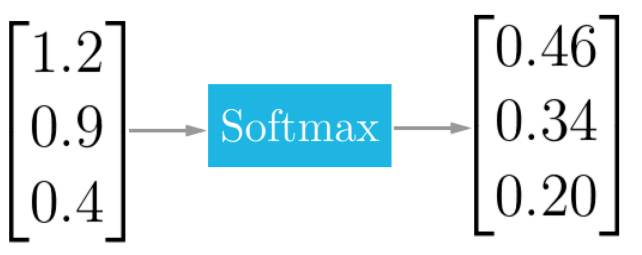
\includegraphics[width=0.7\linewidth]{images/softmax}
	\caption{Klassenzuordnung über Wahrscheinlichkeiten in der Softmax-Konfiguration \cite{Kulbear.2017}} %Generelle
	\label{fig:soft}
\end{figure}
 Die Vorhersagen der Output-Schicht geschieht durch die Funktion $p(j)$. Dabei steht der Index l für die jeweilige Klasse, also die Sprache, die gelernt werden soll.  
\begin{equation}
p(j)= \frac{ exp(x_{j}) }{\sum_{l}{}{ exp(x_{l})} }
\label{eq:soft}
\end{equation}
Für den vorhin erwähnten Gradientenabstiegsverfahren wird ebenfalls eine Kostenfunktion benötigt. Diese geschieht durch Cross-Entropy-Loss-Funktion. 
\begin{equation}
C= \sum_{l}{}{ t_{j} * log(p_{j})} 
\label{eq:back}
\end{equation}
Diese Funktion misst die Abweichungen der Kantengewichte der Netztopologie und passt diese rückwirkend an. Der Cross-Entropy-Verlust nimmt zu, wenn der vorhergesagte Wert von der tatsächlichen Beschriftung abweicht \cite{MLCheatsheet.2017}. Bei $t_{j}$ handelt es sich um die Klasse, für die der Verlust berechnet wird \cite{GonzalezDominguez.2015}.

\subsection{Netztopologie}
Die Netztopologie beschreibt die Infrastruktur des Netzes. Die Auswahl der Topologie bestimmt die Qualität des Trainingsvorgangs. Eine zu geringe Anzahl der Neuronen führt zu einem niedrigen Klassifizierungsrate. Wiederum eine zu hohe Anzahl würde zu Verlängerung des Trainingsdauers führen. Aufgrund dessen fallen Topologien von Ansatz zu Ansatz unterschiedlich aus, welche unterschiedliche Spracherkennungsresultate liefern \cite{bishop.2006}. In dieser Arbeit wird der Topologienvorschlag von Gonzales et al. betrachtet. Für die Eingangsdaten werden 40 Filterbanken verwendet. Diese werden benötigt, um die Daten samplen zu können. In der Input-Schicht werden 26 Neuronen eingesetzt. Um unerwünschte Latenzzeiten zu vermeiden wird ein asymmetrischer Kontext verwendet. Die Hidden-Schicht beträgt vier Ebenen mit einer Gesamtzahl von 2560 Knoten. Die Output-Schicht enthält wie bereits erwähnt eine Softmax-Konfiguration, dessen Dimension der Anzahl der Zielsprachen entspricht. Dies ist bei der Erkennung von multilingualen Sprachen eine erforderliche Konfiguration \cite{GonzalezDominguez.2015}.
 
%\begin{figure*}[h!]
%	\centering
%	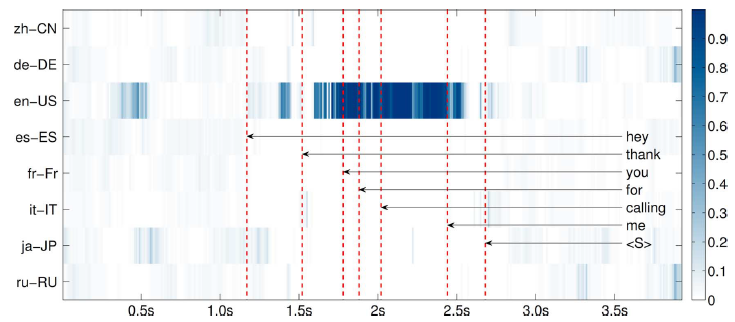
\includegraphics[width=1.0\linewidth]{images/Output}
%	\caption{Netztopologie zur  \cite{GonzalezDominguez.2015}} %Generelle
%	\label{fig:topology}
%\end{figure*}
\subsection{Verbesserung des Trainingsverfahrens durch Multitasking learning (MTL)}
 Bei maschinelles Lernen wird der Fokus gesetzt, bestimmte Metriken, wie beispielsweise Klassifizierungsgenauigkeit und Trainingsdauer, zu optimieren. Daraufhin wird das Modell soweit optimiert, bis die Leistung des Modells nicht mehr gesteigert werden kann \cite{Ruder.2017} \cite{bishop.2006}. Das Lernen der einzelnen Sprachen läuft sequenziell ab. Hier setzt das Multitasking Learning (MTL) ein. Es werden mehrere Lernaufgaben gleichzeitig erledigt statt sequentiell, um das Trainingsvefahren effizienter zu gestalten. Das führt zu einer verbesserten Lerneffizienz und Vorhersagegenauigkeit. Im Klassifizierungskontext zielt MTL darauf ab, die Leistung mehrerer Klassifizierungsaufgaben zu verbessern, indem sie gemeinsam erlernt werden \cite{Lu_multitasklearning}. Ein Beispiel hierfür ist ein Spamfilter. Der Schlüssel zur erfolgreichen Anwendung von MTL besteht darin, dass die Aufgaben miteinander verknüpft werden. Dies bedeutet nicht, dass die Aufgaben ähnlich sein müssen. Stattdessen bedeutet es, dass Aufgaben auf verschiedene Ebenen abstrahiert und geteilt werden. Wenn die Lernaufgaben ähnlich sind, können sie gemeinsam gelernt werden. Dabei kann das Wissen zwischen Aufgaben auf andere Lernaufgaben übertragen werden, welches die Trainingsdauer deutlich verkürzt. MTL ist vor allem dann nützlich, wenn die Größe des Trainingssatzes im Vergleich zur Modellgröße klein ist. Dabei wird grundsätzlich zwei Arten von MTL unterschieden: Hard parameter sharing und soft parameter sharing. \\ \\ Hard parameter sharing stellt das meist genutzte Art dar\cite{Ruder.2017}. Es wird normalerweise auf die Hidden-Schicht angewendet, indem die Aufgaben gemeinsam gelernt werden, während die spezifischen Aufgaben separat gelernt werden. Dies wird in Abbildung \ref{fig:hard} dargestellt. Dieser Ansatz reduziert das Risiko von overfitting erheblich. Je mehr Aufgaben gleichzeitig gelernt wird, desto mehr muss das Modell eine Repräsentation finden, die alle Aufgaben erfassen muss. Dadurch ist die Chance auf overfitting deutlich geringer \cite{Ruder.2017} \cite{Lu_multitasklearning}.
  \begin{figure}[h!]
 	\centering
 	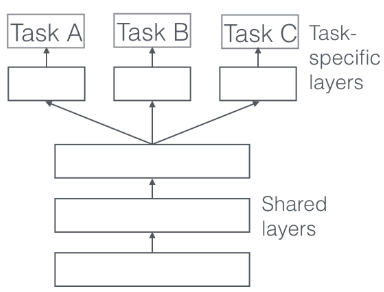
\includegraphics[width=0.8\linewidth]{images/hard}
 	\caption{Hard parameter sharing auf die Hidden-Schicht angewendet \cite{Kulbear.2017}.} %Generelle
 	\label{fig:hard}
 \end{figure}

